\documentclass[a4paper, 15pt]{article}
\usepackage[left=0.85in, right=0.85in, top=0.5in, bottom=0.95in]{geometry}
\usepackage[T1]{fontenc}
\usepackage[utf8]{inputenc}
\usepackage[italian]{babel}
\usepackage[none]{hyphenat} % no sillabazione 
\usepackage{multicol} %testo su più colonne
\usepackage{enumerate}
\usepackage{enumitem}
\usepackage{mdwlist} %suspend enumerate \suspend{} \resume{}
\usepackage{lipsum} %testo random per verifica \lipsum
\usepackage{graphicx, nicefrac}
\usepackage{wrapfig2}
\usepackage{amsmath}
\usepackage{mathtools}
\usepackage{amssymb}
\usepackage{amsthm} %teoremi e dimostrazioni e definizioni
\usepackage{cases}
\usepackage{gensymb} %simboli come ° = \degree  etc etc
\usepackage{cancel} %permette di fare semplificazioni utilizzando il comando \cancel{expression}
\usepackage{subcaption}
\usepackage{hyperref}
\hypersetup{
	colorlinks=true,
	linkcolor=blue,    
	urlcolor=blue,
	%pdfpagemode=FullScreen, %il pdf generato non si avvia a schermo intero
}
\urlstyle{same}
\usepackage{changepage}
\usepackage{lastpage, epstopdf}
\usepackage{fancyhdr}
\usepackage{tcolorbox}
%\usepackage{background} %non utilizza lo sfondo con "draft"
\usepackage{color} % testo colorato \textcolor{'ColorCode'}{'testo'}
\usepackage{setspace} % in questo modo posso settare lo spoazio dell'indice \begin{spacing}{0.95}
	
\usepackage{changepage}
\usepackage{lastpage, epstopdf}
\usepackage{fancyhdr}
\usepackage{tcolorbox}
%\usepackage{background}
\usepackage{tikz} %disegni e mappe
\usetikzlibrary{patterns}
\usepackage{pgfplots}
\pgfplotsset{compat=1.15}
\usepackage{mathrsfs}
\usetikzlibrary{arrows,decorations.markings}
\raggedbottom
\setlength{\parindent}{0pt}
%%%%%%%%%%%%%%%%%%%%%%%%%%%%%%%%%%%%%%%%%%%% SIUNITX 
\usepackage{siunitx}

%========TEOREMI========%
\newtheorem*{thm}{Teorema}
\newtheorem*{en}{Enunciato}
\newtheorem*{definizione}{Definizione}
\newtheorem*{cor}{Corollario}



%========OPERATORI&COMANDI========%
\DeclareMathOperator{\rk}{rk}
\DeclareMathOperator{\im}{Im}
\DeclareUnicodeCharacter{20AC}{\EUR}
\newcommand{\cmark}{\ding{51}}
\newcommand{\xmark}{\ding{55}}
\newcommand{\compresslist}{ % Define a command to reduce spacing within itemize/enumerate environments, this is used right after \begin{itemize} or \begin{enumerate}
				\setlength{\itemsep}{1pt}
				\setlength{\parskip}{0pt}
				\setlength{\parsep}{0pt}
			}
\newcommand{\ra}[1]{\renewcommand{\arraystretch}{#1}} %stretcho le tabelle
			
			%\renewcommand{\arraystretch}{2.5} % Da copiaincollare prima di ambienti array per ampliarli un po'
			%\setlength{\jot}{10pt} % affecting the line spacing in the environment SPLIT
			
\begin{document}
				\setcounterpageref{secnumdepth}{0}	% NON NUMERO I CAPITOLI
				\setcounter{tocdepth}{5} % INCLUDO addirittura I sotto-PARAGRAFI
				\tableofcontents 
				\newpage
				
\part{4.GUM: guide to the expression of uncertainty in measurement}
\section{Introduzione}	
\begin{adjustwidth}{2in}{}
		La GUM definisce le regole per valutare ed esprimere l’incertezza nelle
		misure. \newline
		
		Una misura è un'informazione costituita da un numero, un'incertezza e un'unita di misura:
		\[X = (z \pm u)g\]
		Per cui il risultato di una misurazione altro non è che la stima del valore del misurando che si considera completo solo quando viene accompagnato dalla valutazione
		dell’incertezza legata a tale stima, sempre sotto le ipotesi per cui il misurando deve essere definito con sufficiente completezza in funzione dell'accuratezza richiesta. 
\end{adjustwidth}
%\newpage
\section{Errore vs Incertezza}
\begin{adjustwidth}{2in}{}		
		Il concetto di \textbf{errore} è ben diverso dal concetto di incertezza; l'errore rappresenta la differenza tra il valore misurate ed il valore e può essere sia causale che sistematico. 
		
		Un \textbf{errore casuale} deriva da variazioni stocastiche non conosciute delle grandezze di influenza determinando variazioni nella misura del misurando in presenza di misure ripetute. Questo viene ridotto aumentando il numero di misure sotto le ipotesi che il suo valore medio, il suo valore atteso sia nullo. 
		
		Un \textbf{errore sistematico} è caratterizzato dall'avere media non nulla per cui, se l'effetto di una determinata grandezza di influenza è noto la misurazione può
		essere corretta attraverso un fattore di correzione a cui però si lega un'incertezza.\newline 
		
		L'\textbf{incertezza} è invece un parametro associato al risultato si una misurazione che caratterizza la sua specifica dispersione di valori attribuibili al misurando. 
		
		L'incertezza del risultato di una misurazione riflette così la mancanza di
		conoscenza del valore esatto del misurando, per cui eliminando gli errori sistematici saranno gli errori casuali a determinare l’incertezza
		relativa alla correzione utilizzata.
		
		Alcune fonti di incertezza possono essere l'incompleta e l'imperfetta definizione del misurando, l'inadeguata conoscenza degli effetti delle condizioni ambientali sulla misura, un errore di lettura negli strumenti analogici, una risoluzione degli strumenti non infinita\dots\newline
		
		Le componenti dell'incertezza vengono suddivise in due categorie basate sul metodo di valutazione, la \textit{Tipo A} e la \textit{Tipo B}. Questa classificazione indica due metodi differenti per valutare l’incertezza non
		indicando altresì alcuna differenza tra la natura delle componenti di incertezza, in entrambi i casi infatti l’incertezza è sempre valutata attraverso una distribuzione di
		probabilità e la sua deviazione standard. 
		
		Tale trattazione inoltre non risente di legami con errori di tipo sistematico o casuale.  
\newpage		
		\begin{tcolorbox}[colback=blue!5!white,colframe=blue!75!black,title=TIPO A]
				Ottenuta da una
			funzione di probabilità
			calcolata da dati \\
			Statistica applicata alle misure effettuate
		\end{tcolorbox}
	 	 
	 	 \begin{tcolorbox}[colback=red!5!white,colframe=red!75!black,title=TIPO B]
	 	 	Ottenuta da una
	 	 	funzione di probabilità
	 	 	assunta essere quella reale \\
	 	 	Statistica applicata ad una misura effettuata
	 	 \end{tcolorbox}
\end{adjustwidth}
%\newpage
\section{Valutazione dell’incertezza}
\begin{adjustwidth}{2in}{}	 	 
 	 Come si trova l'incertezza di $Y$ variabile dipendente a partire da quella di $X$ variabile indipendente?
 	 \[Y = f(X_1, X_2, X_3, \dots, X_N)\]
 	 I valori e l'incertezza delle $X_i$ grandezze in ingresso \textbf{O} sono determinate direttamente tramite la misura \textbf{O} hanno origine esterna alla misurazione e i coefficiente sino ottenibili da manuali o certificati di taratura. \newline 
 	 
 	 La stima della misura risulta sempre essere:
 	 \[\overline{Y} = {1\over n}\sum_{k=1}^{n}Y_k = {1\over n}\sum_{k=1}^{n}f(X_{1,k}, X_{2,k}, X_3{3,k}, \dots, X_{N,k})\]
 	  	 	 
 	 Si definisce l'\textbf{incertezza combinata standard} $u_c(Y)$ come funzione delle \textbf{incertezze standard} relative ad ogni grandezza d'ingresso $u(X_i)$. 
 	 	
 	 L'incertezza standard viene anche chiamata incertezza tipo e può esse calcolata sia col metodo \textcolor{blue}{\textbf{A}} che col metodo \textcolor{red}{\textbf{B}}.\newline 
 	 
 	 Considerando sia ogni grandezza in ingresso $X_i$ che $Y$, l’\textbf{incertezza estesa} $U$ è ottenuta moltiplicando l’incertezza combinata standard per un \textbf{fattore di
 	 copertura} $ k $.
  	\[ U(X_i) = ku(X_i) \hspace{1cm} U(Y) = ku_c(Y)\]
 	 Come si sceglie $K$? $ k $ viene scelto in funzione del livello di confidenza richiesto; nel caso di errori della misura a media nulla ed in presenza di un numero
 	 maggiore di 30 misure, il valore di $ k $ coincide con il valore di z della
 	 distribuzione gaussiana:
 	 
 	 \[k=1 \Rightarrow c = 68.3\% \hspace{0.5cm} k=2 \Rightarrow c = 95.5\% \hspace{0.5cm} k=3 \Rightarrow c = 99.7\%\]
	
	Nel caso sempre di errori della misura a media nulla ma in presenza di un numero
	minore di 30 misure, il valore di $ k $ coincide con il valore di $ t $ della distribuzione
	del $ t $ di Student in funzione del numero di gradi di libertà. 
	
	\begin{tcolorbox}[colback=blue!5!white,colframe=blue!75!black,title=TIPO A]
		Comprende quelle incertezze di misura la cui valutazione può
		essere basata su metodi statistici oggettivi.
	\end{tcolorbox}

\begin{tcolorbox}[colback=red!5!white,colframe=red!75!black,title=TIPO B]
	Comprende quelle incertezze la cui stima è basata su “altri
	metodi”, implicando valutazioni di tipo soggettivo.
\end{tcolorbox}
\newpage	
	Come trovare e valutare l'incertezza?
	\begin{enumerate}
		\item Si calcola l'incertezza sulle $X$: come si valutano queste incertezze sulle variabili indipendenti? In che modo influenzano il risultato finale?
		\item Attraverso la propagazione delle incertezze (ex. degli errori) si giunge a capire come le incertezze al punto $1.$ influenzano il risultato sulla variabile dipendente $Y$.
	\end{enumerate}	
	Se durante la misura tutte le grandezze d’influenza
	variano in modo casuale e di conseguenza gli errori della misura hanno
	media nulla con distribuzione gaussiana, il calcolo dell’incertezza può essere effettuato
	utilizzando un approccio statistico \textcolor{blue}{\textbf{TIPO A}}, ma è un'operazione lunga, costosa e non sempre attuabile.  	
	\paragraph{\Large \textcolor{blue}{\textbf{TIPO A}}} \mbox{} \\ 
	La migliore stima del valore vero $\mu$ nel caso di una i-esima grandezza che varia in modo casuale è rappresentata dalla media: 
	\[\overline{X}_i = {1\over n}\sum_{k=1}^{n}X_{i,k}\]
	La deviazione standard di ogni singola misura per l'i-esima grandezza è:
	\[s(X_i) = \sqrt{\dfrac{\sum_{k=1}^{n}\left(X_{i,k}-\overline{X}_i\right)}{n-1}}\]
	La deviazione standard della media dell'i-esima grandezza è: 
	\[s(\overline{X}_i) = {s(X_i)\over\sqrt{n}}\]
	Si definisce l'incertezza standard dell'i-esima grandezza $X_i$ come:
	\[u(X_i) = S(\overline{X}_i)\]
	In modo che l'incertezza estesa associata alla misurazione sia:
	\[U=ku\]
	Chi sceglie $k$? Lo sperimentatore, solitamente per avere valori statisticamente affidabili $k\geq2$.  	
	\paragraph{\Large \textcolor{red}{\textbf{TIPO B}}} \mbox{} \\ 
	L’incertezza stimata con B dà informazioni riguardanti la possibile variabilità della i-esima
	grandezza da misurare.
	
	L'incertezza stimata B risulta più "soggettiva", è lo sperimentatore che assegna il valore all'incertezza. È una tipologia di analisi da utilizzare e preferire quando gli errori delle misure non hanno media nulla e quindi non sono a distribuzione casuale. 
	
	Le informazioni si questa misura possono derivare da dati di misure precedenti, o dalla conoscenza del comportamento dei materiali e degli strumenti, o da note specifiche del costruttore, da certificati o dati di taratura, dall'incertezza assegnata a dati di riferimento in manuali, a previsioni circa variazioni delle grandezze d'influenza\dots 	
	\begin{enumerate}
		\item Si individua un intervallo di valori entro il quale si suppone debbano cadere i valori della i-esima grandezza da misurare.
		\item Si stabilisce una densità di probabilità per ogni fonte di incertezza:
		\begin{itemize}
			\item Distribuzione normale;
			\item Distribuzione rettangolare;
			\item Distribuzione triangolare;
			\item Distribuzione ad U;
		\end{itemize}
		\item Si stima l’incertezza standard della i-esima grandezza da misurare in funzione
		della distribuzione di probabilità che la caratterizza e dà informazioni note “a
		priori”.
	\end{enumerate}
\end{adjustwidth}
%\newpage
\subsection{Distribuzione Normale}
\begin{adjustwidth}{2in}{}
	La distribuzione normale si utilizza quando è maggiore la probabilità di
	trovare valori prossimi al valor medio che lontani da esso. 	
	\begin{figure}[H]
		\centering
		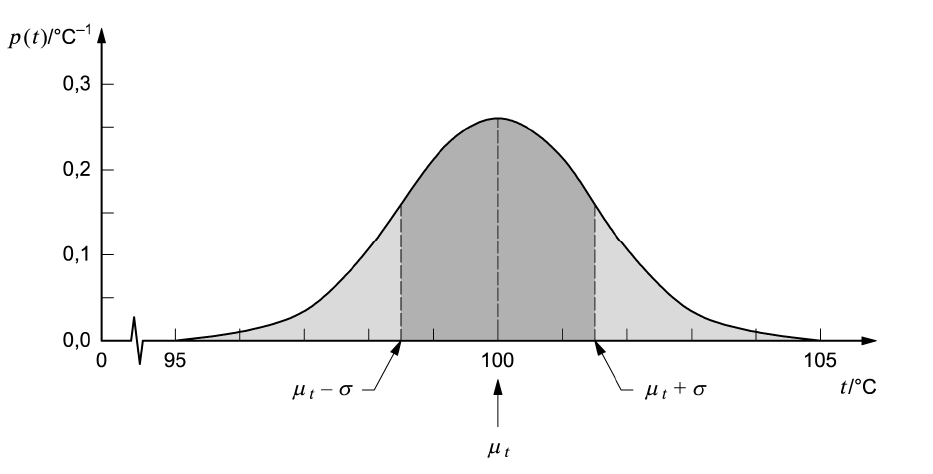
\includegraphics[width=0.5\linewidth]{fig/screenshot001}
		\label{fig:screenshot001}
	\end{figure}
	\[ p(x) = {1\over\sqrt{2\pi}}e^{-{x^2\over2}} \hspace{1cm} \sigma^2(x) = \int_{-\infty}^{+\infty}(x-\overline{x})^2p(x)dx\]
	\[u(x) = \sigma(x) \]
\end{adjustwidth}
%\newpage
\subsection{Distribuzione Rettangolare}
\begin{adjustwidth}{2in}{}	
	La distribuzione rettangolare si utilizza quando si conoscono i limiti di
	variazione del misurando, questo varia in un range di valori finito e definito.
	
	È caratterizzata dal fatto che la probabilità di trovare valori all’interno dell’intervallo è la stessa, questi non si attestano intorno al valor medio. 
	
	Generalmente viene utilizzata nel caso in cui non si abbiano informazioni sulla
	distribuzione all’interno dell’intervallo.\newline
	
	Le equazioni che individuano questa distribuzione sono:
	\[\begin{matrix}		
			p(x) = \dfrac{1}{2a} & a_- \leq x \leq a_+ \\
			p(x) = 0 & x<a_- ~ x>a_+		
	\end{matrix}\]
    In cui $a$ è il semi intervallo di valori possibili.
    
    Per far valere il fatto che la sua area sia unitaria, ovvero che debba abbracciare una probabilità del 100\%, le dimensioni del rettangolo dovranno esser pari a:
    \[A = b\cdot h = 2a\cdot{1\over2a} = 1\]   
    \begin{figure}[H]
    	\centering
    	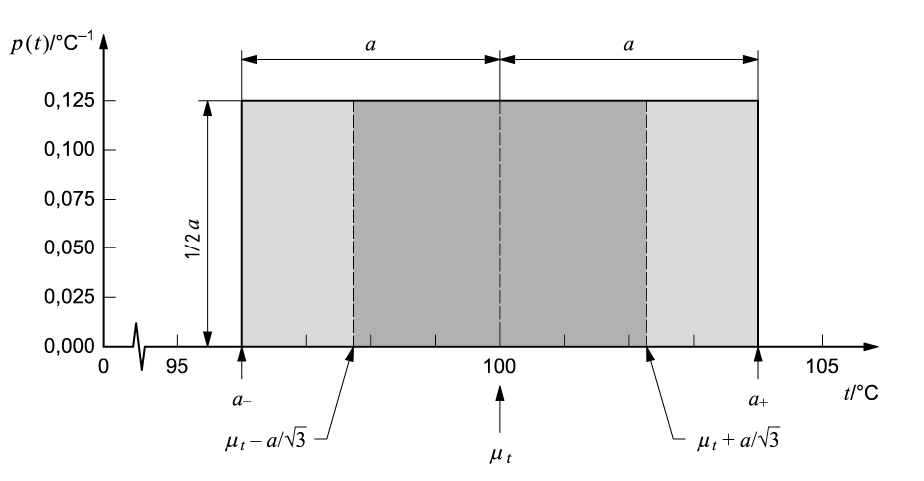
\includegraphics[width=0.7\linewidth]{fig/screenshot002}
    	\label{fig:screenshot002}
    \end{figure}  
\newpage
	In questo caso, svolgendo l'integrale ottengo:
	\[u(x) = \sigma(x) = {2a\over\sqrt{12}} = {a\over\sqrt{3}}\]
	 L'area evidenziata in grigio identifica cosi i valori di $\pm u(x)$. \newline
	 
	 Che valori si scelgono di $k$? Scegliendo $k=2$ ottengo:
	 \[ U = \pm 2u = \pm{2a\over\sqrt{3}} \] 
	 Sto sovradimensionando l'incertezza, sto andando oltre la distribuzione di probabilità definita, al massimo si può scegliere $k = \sqrt{3}$, in questo modo 
	  \[ U = \pm \sqrt{3}u = \pm a  \]
	  Deve essere perciò $k\leq\sqrt{3}$ per $k=1$ l'area racchiusa è il 59\%. \newline
	  
	  Quando si usa questa distribuzione? La risoluzione degli strumenti digitali ne è un classico esempio, si ha infatti ad esempio, la seguente misura di una grandezza, $1.28$ per cui non si conosce la cifra decimale, per cui quale potrebbe essere?
	  \[ 1.280 ~ 1.282 ~ 1.277 \]
	  Queste ad esempio sono tutte plausibili, si ha la stessa probabilità di vere una misura tra queste, ma cosa sicuramente si esclude? Si esclude la possibilità che sia $1.286$ perché altrimenti sullo strumento si leggerebbe $1.29$ anziché $1.28$, per cui, qual è il limite? 
	  \[ 1.275<1.28<1.285\]
	  In questo modo $a$ si configura essere:
	  \[a = \dfrac{\text{minimo scarto}}{2}\]
	  E perciò in questo caso, avendo l'incertezza sul decimo, si avrà:
	  \[a = \dfrac{0.01}{2} 0.005\]
	  E quindi, l'incertezza associata a tale semi intervallo sarà:
	  \[u = {a\over\sqrt{3}}= {0.005\over\sqrt{3}} = 0.0028\]
	  
	  Un altro classico esempio di distribuzione rettangolare è la tolleranza dimensionale.  
\end{adjustwidth}
\newpage
\subsection{Distribuzione Triangolare}
\begin{adjustwidth}{2in}{}	  
	  La distribuzione triangolare si utilizza qualora vi sia maggiore probabilità di
	  trovare valori prossimi alla media piuttosto che lontano da essa.
	  
	  Si ipotizza una variazione lineare tra la media ed i limiti, per cui le equazioni che la identificano sono: 
	  \[\begin{matrix}
	  	p(x) = \dfrac{x-a_-}{a^2} & a_- \leq x \leq {a_+ + a_-\over2} \\
	  	p(x) = \dfrac{a_+-x}{a^2} &  {a_+ + a_-\over2} \leq x \leq a_+ \\
	  	p(x) = 0 & \text{altrimenti}
	  \end{matrix}\]
  		\begin{figure}[H]
  			\centering
  			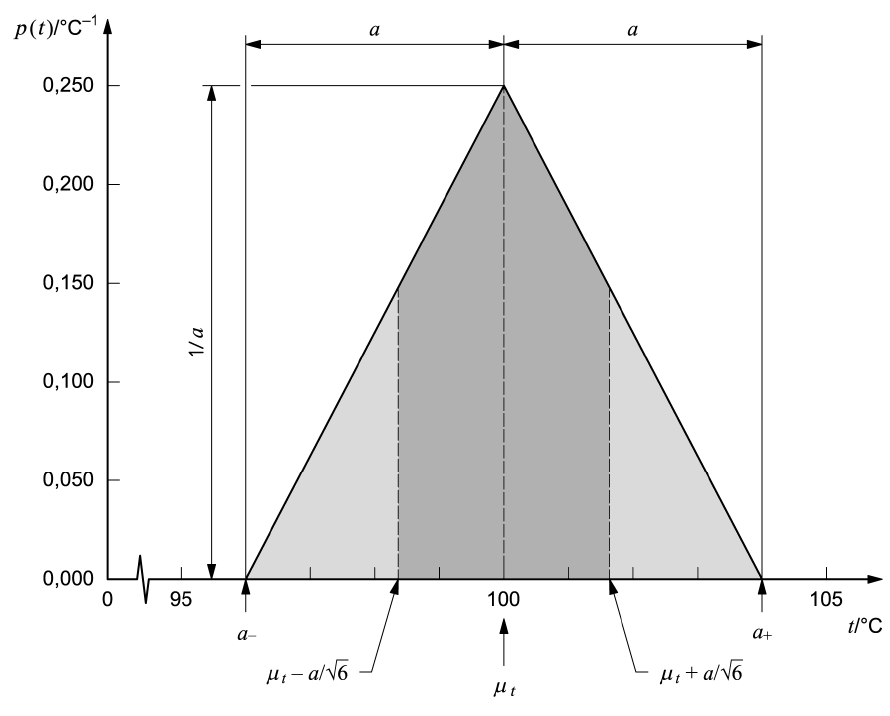
\includegraphics[width=0.5\linewidth]{fig/screenshot003}
  			\label{fig:screenshot003}
  		\end{figure}
  		Per cui: 
  		\[u(x) = \sigma(x) = {a\over\sqrt{6}}\]
  		 questa è una distribuzione a metà, a cavallo tra quella gaussiana e quella rettangolare, perché identifica i valori centrali come i più probabili ed è limitata. \newline 
  		 
  		 In questo caso $k\leq\sqrt{6}$ per cui $k=1$ identifica un'area pari al 41\%.  
\end{adjustwidth}
\newpage
\subsection{Distribuzione ad U}
\begin{adjustwidth}{2in}{}  		 
  		 La distribuzione ad “U” è utilizzata quando è maggiore la probabilità di trovare
  		 i valori misurati vicino ai limiti piuttosto che intorno al valore medio.
  		 
  		 Tale distribuzione è usata ad esempio in meteorologia, dove il malore medio non è rappresentativo, si danno valori minimi e valori massimi. 
  		 
  		 Anche le vibrazioni fanno uso di questa distribuzione, hanno andamenti sinusoidali spesso a media nulla identificati da un minino ed un massimo.  	
  		 \begin{figure}[H]
  		 	\centering
  		 	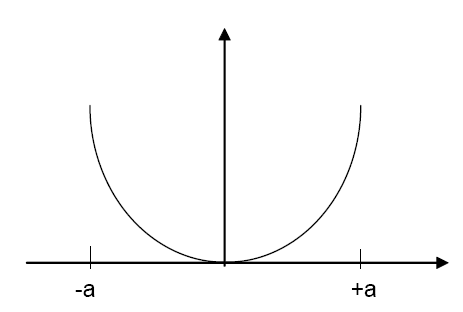
\includegraphics[width=0.5\linewidth]{fig/screenshot004}
  		 	\label{fig:screenshot004}
  		 \end{figure}  		   		 
  		 In questo caso, poiché:
  		 \[u(x) = {a\over\sqrt{2}}\]  
  		 Allora $k\leq\sqrt{2}$
\paragraph{Ricapitolando} i contributi all’incertezza combinata standard possono essere calcolati tramite
  		 i metodi \textcolor{blue}{\textbf{TIPO A}} e \textcolor{red}{\textbf{TIPO B}}. Infatti si possono avere due situazioni limite:
  		 \begin{enumerate}
  		 	\item Singola misurazione – non è possibile stimare le incertezze di tipo A, si considerano
  		 	unicamente quelle di tipo B;
  		 	\item Numerose misurazioni – tutte le grandezze di influenza vengono fatte variare in
  		 	modo casuale per stimare le cause di incertezza unicamente tramite metodo A;
  		\end{enumerate}
  		Si stabilisce infine il fattore di copertura e si fornisce il valore dell’incertezza estesa
  		per ogni i-ma grandezza.
  		
  		Si noti infine come il fattore moltiplicativo $k$ è maggiore nella distribuzione "U" piuttosto che nella distribuzione rettangolare e triangolare. \newline 
\end{adjustwidth}
\newpage
\section{Propagazione delle incertezze}
\begin{adjustwidth}{2in}{}    		
  		L’incertezza composta si usa in presenza di misure indirette ossia dove è presente
  		un legame funzionale tra le grandezze misurate $X_i$ ed il parametro di cui si
  		vuole conoscere la misura $Y$:
  		\[Y = f(X_1, X_2, X_3, \dots X_N)\]
  		L’incertezza composta è una stima della dispersione dei valori di $ Y $ a causa
  		delle incertezze associate a $X_i$. Le incertezze standard possono essere di \textcolor{blue}{\textbf{TIPO A}} e di \textcolor{red}{\textbf{TIPO B}} e le grandezze misurate possono essere tra di loro indipendenti o correlate.  
\end{adjustwidth}
%\newpage
\subsection{Grandezze misurate indipendenti}
\begin{adjustwidth}{2in}{}   		
  		Valendo solamente se le grandezze sono tra di loro indipendenti, ovvero se ad esempio \( y=f(x_1, x_2, x_3) ~ \nexists ~ x_1 = f(x_2)\) si effettuano le derivate parziali rispetto alle singole variabili:
  		\[ u_c(y) = \sqrt{\sum_{i=1}^{N}\left(\partial f\over\partial x_i\right)^2\cdot u^2(x_i)}\]
  		Dove la $u(x_i)$ sarà l'incertezza di tipo A o B per ogni variabile.\newline 
  		
  		Ad esempio se:
  		\[y = a + b + c \Rightarrow {\partial f\over\partial a} = 1 \quad {\partial f\over\partial b} = 1 \quad {\partial f\over\partial c} = -1 \]
  		Allora:
  		\[u_c(y) = \sqrt{1\cdot u_a^2 + 1\cdot u_b^2 + 1\cdot u_c^2}\]
\end{adjustwidth}
%\newpage
\subsection{Grandezze misurate correlate}
\begin{adjustwidth}{2in}{}     		
  		\[ u^2_c(y) = \sum_{i=1}^{N}\left(\partial f\over\partial x_i\right)^2\cdot u^2(x_i) + 2\sum_{i=1}^{N-1}\sum_{j=i+1}^{N} {\partial f\over\partial x_i}\cdot{\partial f\over\partial x_j}u(x_i)u(x_j)\cdot r(x_i, x_j)\]
  		In cui $r$ è il fattore di correlazione: 
  		\[ r(x_i, x_j) = \dfrac{u(x_i, x_j)}{u(x_i)\cdot u(x_j)}\]
  		In cui $u(x_i, x_j)$ è la covarianza tra $x_i$ e $x_j$:
  		\[u(x_i, x_j) = {1\over n}\sum_{k=1}^{n}(x_i-\overline{x}_i)(x_j-\overline{x}_j)\]
  		Per cui se $r=0$ non c'è correlazione e se $r=1$ c'è correlazione.  
\end{adjustwidth}
\newpage
\subsection{Esempio - Misura di una resistenza nel partitore di tensione}
\begin{adjustwidth}{2in}{}  		
\begin{figure}[H]
	\centering
	\label{fig:screenshot005}
	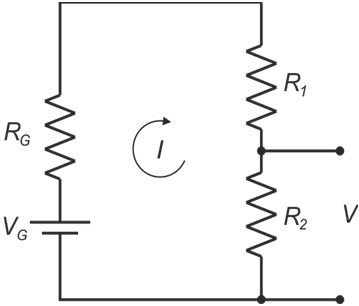
\includegraphics[width=0.3\linewidth]{fig/screenshot005}
\end{figure}
  		\[R_2 = \dfrac{V}{V_G-V}(R_G+R_1)\]
  		\begin{enumerate}
  			\item $ V_G=12V $ tensione di alimentazione con incertezza estesa $ U(V_G)=10mV (k=2) $
  			\item $ R_G=10\Omega $ misurata tramite 10 letture, la deviazione standard è $ 12,65 \Omega $
  			\item $ R_1=1k\Omega $ e $ u(R_1)=5\Omega $
  			\item $ V=7,77V $ misurata tramite voltmetro a 3 cifre (presente unicamente l’errore di
  			quantizzazione a distribuzione rettangolare)
  		\end{enumerate}
  		Si chiede di 
  		\begin{itemize}
  			\item Calcolare l’incertezza assoluta per tutti i parametri
  			\item Calcolare il valore di $ R_2 $
  			\item Calcolare l’incertezza combinata standard di $ R_2 $
  			\item Calcolare l’incertezza estesa di $ R_2 $  		
  		\end{itemize}
  		Si procede a dare la soluzione:
  		\[ \begin{array}{c}
  			\begin{aligned}
  				u(R_1) & = u(R_1)=5\Omega ~ \text{nota} \\
  				u(R_G) & = {\sigma\over\sqrt{n}} = {12,65\over\sqrt{10}} = 4\Omega \\
  				u(V_G) & = {U(V_G)\over k} = 10mV/2 = 5mV \\
  				u(V)  & = {a\over\sqrt{3}} = {\left(0.01\over2\right)\over\sqrt{3}} = {0.005\over\sqrt{3}} = 2.29mV \\
  				R_2 & = \dfrac{7.77}{12-7.77}(10+1000) = 1855\Omega  					
  			\end{aligned}
  		\end{array}
  		 \]
  		 L'incertezza combinata standard su $R_2$ si trova tramite l'ottenimento delle derivate parziali:
  		\end{adjustwidth}
  		 \[ \begin{array}{c}
  		 	\begin{aligned}
  		 		{\partial R_2\over\partial R_1} & = \dfrac{V}{V_G-V} = 1.84 mV  \\
  		 		{\partial R_2\over\partial R_G} & = \dfrac{V}{V_G-V} = 1.84 mV \\
  		 		{\partial R_2\over\partial V_G} & = \dfrac{V_G(R_G+R_1)}{(V_G-V)^2}  = 667.3  \\
  		 		{\partial R_2\over\partial V} & =  -\dfrac{(R_G+R_1)}{(V_G-V)^2} = 438.6 \\
  		 		
  		 		 \left({\partial R_2\over\partial R_1}\right)^2 = 3.38; ~ \left({\partial R_2\over\partial R_G}\right)^2 & = 3.38; ~ \left({\partial R_2\over\partial V_G}\right)^2 = 458821; \left({\partial R_2\over\partial V}\right)^2 = 192369.96 \\  
  		 		 
  		 		  \left({\partial R_2\over\partial R_1}\right)^2(R_1)^2 = 84.5 ; ~ \left({\partial R_2\over\partial R_G}\right)^2u(R_G)^2 & = 61.82 ; ~ \left({\partial R_2\over\partial V_G}\right)^2u(V_G)^2 = 11.47 ; ~ \left({\partial R_2\over\partial V}\right)^2u(V)^2 = 1.61 ;
  		 	\end{aligned}
  		 \end{array}
  		 \]
  		 In questo modo:
  		  		 
  		 \[ 
  		 	u_c(R_2)  =\sqrt{\left({\partial R_2\over\partial R_1}\right)^2\cdot u(R_1)^2 + \left({\partial R_2\over\partial R_G}\right)^2\cdot u(R_G)^2 + \left({\partial R_2\over\partial V_G}\right)^2\cdot u(V_G)^2 + \left({\partial R_2\over\partial V}\right)^2\cdot u(V)^2 } = \sqrt{165.4} = 12.86\approx 12\Omega
  		 \]
  		 \begin{adjustwidth}{2in}{} 
  		 In più, se $k=2$ sia avrà:
  		 \[U(R_2) = 24\Omega\]  		 
\end{adjustwidth}
\newpage
\section{Propagazione delle distribuzioni: Simulazione Monte Carlo}  		 
\begin{adjustwidth}{2in}{}  
  		 Cosa succede se però non è noto il legame funzionale tra le grandezze misurate
  		 $x_i$ ed il parametro di cui si vuole conoscere la misura $y$?
  		 ovvero non è nota la:
  		 \[y = f(x_N)\]
  		 o è molto difficile da ricavare.
  		 
  		 Si utilizza il supplemento alla GUM (JCGM 101:2008) basato sulla
  		 propagazione delle distribuzioni tale Supplemento raccomanda di implementare detta propagazione delle
  		 distribuzioni mediante la Simulazione Monte Carlo. \newline 
  		 
  		 La propagazione delle distribuzioni va utilizzata quando:
  		 \begin{itemize}
  		 	\item Il modello funzionale devia fortemente dalla linearità;
  		 	\item Le derivate parziali sono difficilmente calcolabili;
  		 	\item Le distribuzioni di probabilità associate alle grandezze da misurare non sono
  		 	gaussiane;
  		 	\item La propagazione delle incertezze fornisce una sovrastima dell’incertezza associata
  		 	alla misura finale (dello stesso ordine della variabile analizzata);
  		 	\item Modello funzionale non noto; 
  		 	\item Modello funzionale complesso (logaritmo, ecc).
  		 \end{itemize} 
  	 
  	 		Per cui, nota la media e la deviazione standard che si vuole avere, si chiede al calcolatore di generare un numero di misure simulate, fittizie, tali per cui la media e la deviazione standard siano uguali al valore imposto. Una volte ottenute tali misure si inseriscono all'interno dell'equazione funzionale di partenza dalla quale si crea una funzione cumulativa della distribuzione, a questo punto si può finalmente dare un valore alla confidenza. \newline 
  	 		
  	 		Che tipo di distribuzione ci si aspetta? Se sono ognuna di tipologia diversa non si è in grado di stabilirlo devono essere tutte uguali per stabilirlo a priori. \newline
  	 		
  	 		La simulazione Monte Carlo procede per step per cui è necessario:
  	 		\begin{enumerate}
  	 			\item Selezionare un numero $ M $ di simulazioni (di solito $ 10^6 $);
  	 			\item Generare $ M $ vettori di numeri per le variabili $ X_i $ tenendo in considerazione la funzione
  	 			di distribuzione di probabilità associata ad ogni $ X_i $;
  	 			\item Per ogni vettore calcolare la relazione funzionale di partenza:
  	 			\[y_k = g(x_{1,k}, x_{2,k},\dots x_{N,k})\hspace{0.5cm} k=1\dots M \] 
  	 			\item Ordinare gli $ M $ elementi di $ y $ in ordine non decrescente ($\approx$ crescente, potrebbero esserci termini uguali);
  	 			\item Costruire la $ F_y $ come conteggio progressivo normalizzato al numero totale
  	 			dell’insieme $ y(k) $; \newline
  	 			\begin{table}[H]
  	 				\centering
  	 				\begin{tabular}{|c|c|}
  	 				\hline
  	 				x & y \\
  	 				\hline
  	 				$ R_{2;\min} $ & 1/M \\
  	 				\hline
  	 				. & 2/M \\
  	 				\hline
  	 				. & 3/M \\
  	 				\hline
  	 				. & .\\
  	 				\hline
  	 				. & . \\
  	 				\hline
  	 				$ R_{2;\max} $ & 1 \\
  	 				\hline
  	 			\end{tabular}
  	 			\end{table}
  	 			\item Calcolare la media e la deviazione standard di $ y $;
  	 			\item L’intervallo di copertura $ [y_1, y_2] $ correlato ad una probabilità di copertura $ p $, è il più
  	 			piccolo intervallo $ [y_1, y_2] $ per cui:
  	 			\[F_y(y_2) - F(y_1) = p\]
  	 		\end{enumerate}
\end{adjustwidth}
\newpage
\subsection{Esempio - Misura di una resistenza nel partitore di tensione}
\begin{adjustwidth}{2in}{}    		
   		\begin{enumerate}
   			\item \[R_2 = \dfrac{V}{V_G-V}(R_G+R_1)\hspace{1cm} M=10^6\]
   			\item Per ogni variabile nota la distribuzione di probabilità si calcola il vettore
   			numerico corrispondente.  			
   			\begin{figure}[H]
   				\centering
   				\label{fig:screenshot006}
   				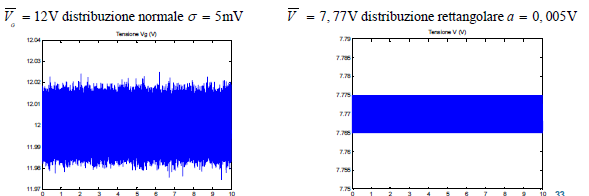
\includegraphics[width=0.5\linewidth]{fig/screenshot006}
   			\end{figure}
   			
   			 \begin{figure}[H]
   			 	\centering
   			 	\label{fig:screenshot007}
   			 	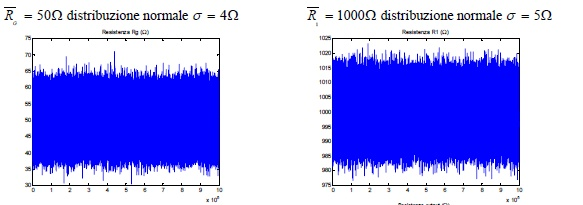
\includegraphics[width=0.5\linewidth]{fig/Inkedscreenshot007}
   			 \end{figure}
   			\item Per ogni valore ottenuto si calcola la
   			resistenza $ R_2 $  			
   			\begin{figure}[H]
   				\centering
   				\caption{}
   				\label{fig:screenshot008}
   				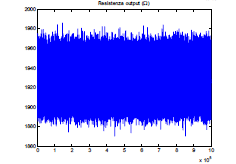
\includegraphics[width=0.5\linewidth]{fig/screenshot008}
   			\end{figure}  			
   			\item[4. + 5.] Dopo aver ordinato i valori di $ R_2 $ in modo non decrescente si
   			costruisce la $ F_R $ avente in ascissa i valori di $ R_2 $ ed in ordinata l’indice
   			normalizzato,
 \begin{figure}[H]
 	\centering
 	\label{fig:screenshot009}
 	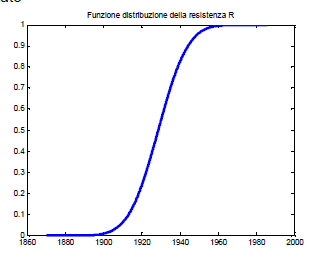
\includegraphics[width=0.5\linewidth]{fig/screenshot009}
 \end{figure}
   			\item[6.]  Si passa al calcolo della media e della deviazione standard di $ R_2 $:
   			\[\overline{R}_2 = 1928.7\Omega \hspace{1cm} \sigma(R_2) = 12.2\Omega\]
   			
   			\item[7.] Infine si calcola l’intervallo di copertura $ [R_{2,\min}, R_{2,\max}] $, correlato ad una
   			probabilità di copertura $ p $, come il più piccolo intervallo $ [R_{2,\min}, R_{2,\max}] $
   			per cui $ F_R(R_{2,\max})-F(R_{2,\min} ) = p $
\begin{figure}[H]
	\centering
	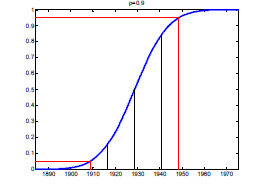
\includegraphics[width=0.5\linewidth]{fig/screenshot010}
	\label{fig:screenshot010}
\end{figure}
   			Si fissi perciò una confidenza:
   			\[100\% \Rightarrow [R_{2,\min}, R_{2,\max}] \]
   			Più realisticamente:
   			\[ 90\% \Rightarrow 0.9\]
   			Si scandagliano con questo valore tutti gli intervalli possibili alla ricerca della media 
   			\[
   				[0; 0.9] \rightarrow \left[1945; 1870\right] \hspace{0.5cm }
   				[0.001; 0.91] \rightarrow \left[1902; 1949 \right] \hspace{0.5cm } 				
   				[0.1; 1] \rightarrow [1985; 1918]
   			\]
   			
   			Dove varia il $\Delta R$? Dove sarà maggiore o minore? Sarà massimo agli estremi e minimo nella zona centrale, in questo modo si prende l'intervallo minimo calcolato, nell'area così sottesa si identificherà una probabilità pari al 90\%.
   			
   			Tale curva ad S è bene notare che cresce rapidamente nella zona centrale, è dunque lì che si si aspetterà la media, inoltre tale curva è ad S se le distribuzioni di partenza sono tutte gaussiane, come cominciano ad essere tutte rettangolari, si linearizza dal valore minimo al valore massimo.  
   		\end{enumerate}   	
   	\begin{figure}[H]
   		\centering
   		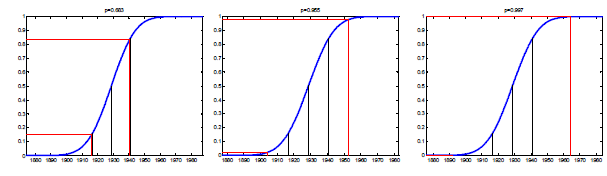
\includegraphics[width=0.8\linewidth]{fig/screenshot011}
   		\label{fig:screenshot011}
   	\end{figure}
\end{adjustwidth}
\newpage
\section{Esprimere l'incertezza}
\begin{adjustwidth}{2in}{}   	
   		Per esprimere l'incertezza bisogna: 
   		\begin{itemize}
   			\item Descrivere chiaramente il metodo usato per calcolare il risultato della misura
   			e l’incertezza correlata (GUM 7.1.4 a);
   			\item Riportare una lista contenente tutte le componenti dell’incertezza e come
   			esse sono state calcolate (GUM 7.1.4 b)
   			\item Nel caso di incertezza estesa $ U(Y) = ku_c(Y) $ bisogna (GUM 7.2.3):
   			\begin{itemize}
   				\item Fornire una descrizione esaustiva di come il parametro $ x $ è definito;
   				\item Riportare il risultato della misurazione come $Y = \overline{Y} \pm U$ fornendo l’unità di misura;
   				\item Fornire l’incertezza estesa relativa pari a $\dfrac{U}{|Y|}$;
   				\item Riportare il valore di $ k $;
   				\item Fornire il livello di confidenza approssimato associato con l’intervallo $ \pm U $ e come è
   				stato calcolato;    				
   			\end{itemize}
   			\item Se si misurano due grandezze contemporaneamente, oltre alla misura e alle
   			incertezze relative ad ogni parametro, bisogna fornire la covarianza ed il
   			coefficiente di correlazione (GUM 7.2.5)
   		\end{itemize}
\end{adjustwidth}
%\newpage
\subsection{Taratura}
\begin{adjustwidth}{2in}{}   	
\textbf{Come si associa l'incertezza alla taratura? }
   		
   		La taratura è quell'insieme di operazioni che stabiliscono, sotto condizioni specificate, la
   		relazione tra i valori indicati da uno strumento - o da un sistema per
   		misurazione - o i valori rappresentati da un campione materiale, ed i
   		corrispondenti valori noti di un misurando [V.I.M., 6.13], per cui \textbf{Tarare uno strumento} significa stabilire una relazione tra le indicazioni
   		fornite dallo strumento ed i valori di un misurando precedentemente determinati con altri metodi di misura, \textbf{Tarare un campione materiale} significa stabilire invece la relazione che intercorre
   		tra il valore nominale del campione e il valore di un misurando
   		precedentemente misurato con altri metodi. 
   		\[y = F(x)\]   		
   		\begin{figure}[H]
   			\centering
   			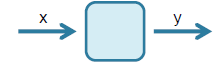
\includegraphics[width=0.2\linewidth]{fig/screenshot012}
   			\label{fig:screenshot012}
   		\end{figure}   		
   		La relazione $F(X)$ rappresenta la modellizzazione del comportamento dello strumento di misura, questa è noto che possa essere espressa tramite un polinomio troncato al primo ordine evidenziando così un comportamento lineare tra ingesso e uscita tramite la retta di regressione. 
   		\[y = F(x) = a+bx\] 		
   		In un misurazione l’incertezza da associare alla misura è legata anche alle
   		incertezze dovute a:
   		\begin{itemize}
   			\item Caratteristiche metrologiche della strumentazione nella catena di misura;
   			\item Effetto delle grandezze di influenza sulla strumentazione;
   			\item Metodo di misurazione o prova;
   			\item Qualificazione del personale;
   		\end{itemize}
\newpage
   		Nel processo di taratura l’incertezza da associare allo strumento in taratura è
   		legata anche alle incertezze dovute a:
   		\begin{itemize}
   			\item Strumento tarante;\newline 
   			I valori dello strumento tarato sono calcolati attraverso uno strumento che possiede intrinsecamente una sua incertezza, come nell'esempio che era stato fatto ad inizio corso della massa campione che propagava la sua incertezza.
   			
   			Ogni strumento tarato ingloba l'incertezza dello strumento tarante, a catena.
   			\item Caratteristiche metrologiche della strumentazione nella catena di taratura;
   			\item Grandezze d'influenza; 
   			\item Processo di taratura;
   			\item Effetto delle grandezze di influenza sullo strumento in taratura, sullo strumento
   			tarante, su ogni elemento del setup di taratura;
   			\item Qualificazione del personale;
   		\end{itemize}
   		Ogni componente della catena di misura possiede una sua incertezza. 
   		\newline 
   		
   		L'incertezza legata all'operazione di taratura viene calcolata conoscendo 
   		\begin{itemize}
   			\item L'\textbf{incertezza del misurando} $u_m$, legata all'imperfetta realizzazione o definizione del misurando;
   			\item l'\textbf{incertezza della strumentazione} $u_{st}$, legata ad ogni elemento appartenente alla catena;
   			di misura (lettura analogica, risoluzione, incertezza strumento tarante, ecc.)
   			\item l'\textbf{incertezza del protocollo} $u_p$, legata ad approssimazioni del metodo di misura;
   			\item l'\textbf{incertezza di interpolazione} $u_{int}$ deriva dalla relazione funzionale che si è deciso di usare per collegare ingresso e uscita, è legata agli algoritmi matematici utilizzati in
   			fase di taratura (retta di regressione, ecc.).
   			\[u_{int} = \sqrt{\dfrac{\sum_{i=1}^{n}M_i^2}{n-m}} \hspace{1cm} M_i = \dfrac{y_{rif, i}-\hat{y}_i}{\left.\dfrac{dy}{dx}\right|_i}\]
   			In cui $n$ è il numero di punti di taratura, $m$ è il numero di coefficienti del polinomio, dei vincoli che si applicano e $dx/sy$ è la derivata calcolata nel punto i-esimo. \newline 
   			
   			Per una regressione lineare i punti $\hat{y}$ sono i valori che assume la retta in quei punti, sono i valori stimati (dalla retta), perciò la differenza $ (y_{rif, i}-\hat{y}_i) $ altro non è che la distanza verticale tra il punto sperimentale e lo stesso punto stimato dalla retta. 
   			
   			La differenza $(n-m)$ invece indica nient'altro che i gradi di libertà del sistema. \newline 
   			
   			Per una relazione lineare si arriva così a:
   			 \[u_{int} = \sqrt{\dfrac{\sum_{i=1}^{n}(y_{rif, i}-\hat{y}_i)^2}{b(n-2)}}\]   			
   		\end{itemize}
\newpage
   		L'incertezza è sul misurando e come si è appena visto può essere causata da molti fattori, ci si pone di identificare allora una sola incertezza, \textbf{incertezza combinata standard di
   			taratura} $u_t$, che si calcola considerando tutte le i-esime cause di incertezza
   		\[u_t = \sqrt{\sum_{i}^{k}u_i^2} = \sqrt{u_m^2 + u_{st}^2 + u_p^2 + u_{int}^2 6 \dots + u_i^2}\]
   		Le incertezze standard coincidono con le $\sigma/N$ se le singole incertezze possono
   		essere considerate tutte distribuite intorno alla media secondo una gaussiana. \newline 
   		
   		L'incertezza estesa $U_{BMC}$ \textit{(Best Measurement
   		Capability} si calcola attraverso il fattore di confidenza $k$ ad un valore definito di confidenza. 
   	
   		Se non sono rispettate le ipotesi del teorema del limite centrale si applica il fattore $k$ legato ai valori ricavati dalla distribuzione $ t $. 
\end{adjustwidth}
%\newpage
\subsubsection{Taratura di un multimetro}
\begin{adjustwidth}{2in}{}    		
   		Nell'esempio di taratura numerale da parte di Accredia, si vede come l'incertezza finale sia largamente governata dal fattore maggiormente preponderante   		
   		\begin{figure}[H]
   			\centering
   			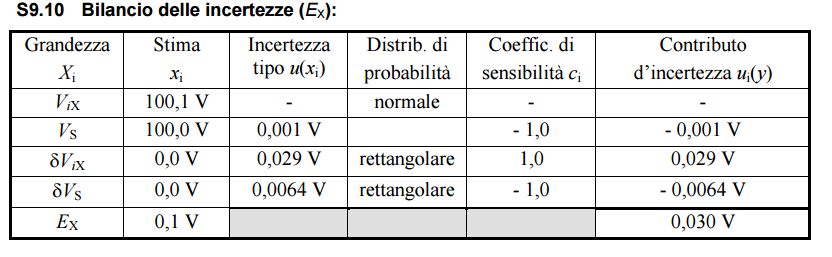
\includegraphics[width=0.5\linewidth]{fig/screenshot013}
   			\label{fig:screenshot013}
   		\end{figure}
\end{adjustwidth}
%\newpage
\subsubsection{Taratura di un calibro}
\begin{adjustwidth}{2in}{}    		
   		Nell'esempio di taratura di un calibro a nonio con blocchetti pian paralleli, si considererà anche l'incertezza dovuta alla variazione di temperatura \(L\alpha\Delta T\) tra il calibro e il blocchetto e una correzione $I_M$ dovuta ad effetti meccanici, come la forza di misura applicata, errori di piattezza e parallelismo e di chiusura.\newline 
   		
   		È un chiaro esempio di come sia necessario considerare tutti gli elementi che fanno parte della catena di misura. \newline 
   		
   		Anche in questo caso si evidenzia che l'incertezza dal valore maggiore governerà per larga parte l'incertezza finale.  		
\begin{figure}[H]
	\centering
	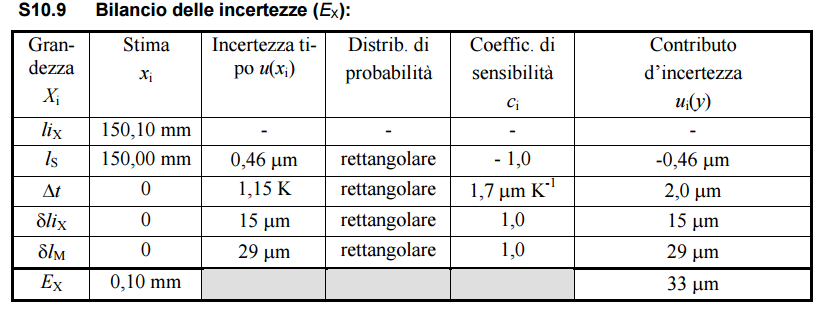
\includegraphics[width=0.5\linewidth]{fig/screenshot014}
	\label{fig:screenshot014}
\end{figure}
   		I servizi di taratura in Italia prima del 2010 venivano svolti dal SIT, Servizio di Taratura. Dal 2010 il servizio di taratura e di accreditamento viene svolto unicamente
   		da ACCREDIA. 
   		
   		ACCREDIA è l'Ente unico nazionale di accreditamento designato dal
   		Governo italiano, opera sotto la vigilanza del Ministero dello sviluppo economico ed è l'unico ente riconosciuto in Italia ad attestare che gli
   		organismi di certificazione ed ispezione, i laboratori di prova e quelli di taratura abbiano le competenze per valutare
   		la conformità dei prodotti, dei processi e dei sistemi agli standard di
   		riferimento.
   		
   		Ogni Paese europeo ha il suo Ente di accreditamento. L'Ente Nazionale è
   		responsabile per l'accreditamento in conformità agli standard internazionali
   		della serie ISO 17000 e alle guide e alla serie armonizzata delle norme
   		europee EN 45000. Tutti gli Enti operano senza fini di lucro.\newline 
   		
   		Le attività dell'Ente si articolano in quattro Dipartimenti: Certificazione ed ispezione, Laboratori di prova, laboratori di prova per la sicurezza degli alimenti, laboratori di taratura. \newline 
   		
   		Ogni centro Accredia fornisce dei servizi e le massime incertezze raggiungibile dalle loro strumentazioni di taratura.    		
\begin{figure}[H]
	\centering
	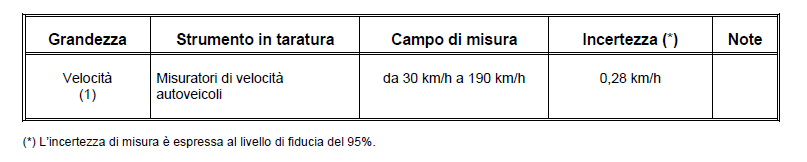
\includegraphics[width=0.5\linewidth]{fig/screenshot015}
	\label{fig:screenshot015}
\end{figure}  		
   		NB: Notare come il campo di misura COINCIDA col campo di taratura, d'altro canto il campo di misura identifica il campo di utilizzo dello strumento, quindi quando si tara uno strumento si definisce automaticamente il suo campo di misura. 
\end{adjustwidth}
%\newpage
\section{Riferibilità}
\begin{adjustwidth}{2in}{}     		
   		Proprietà del risultato di una misurazione consistente nel poterlo riferire a
   		campioni appropriati, generalmente nazionali o internazionali, attraverso una
   		catena ininterrotta di confronti [V.I.M., 6.12].
   		
   		Proprietà che un dispositivo per misurazione e/o regolazione acquisisce
   		quando viene sottoposto a taratura impiegando misurandi le cui misure sono
   		state assegnate con riferimento a campioni riconosciuti come primari in un
   		determinato contesto [UNI 4546, 7.1.1].\newline 
   		
   		Adottando un campione unico a livello nazionale, tutti gli operatori che
   		eseguono misure con riferibilità al campione adottato sono in grado di
   		eseguire misure tra loro compatibili e confrontabili.\newline
   		
   		Se il campione ha però una sua incertezza, quello tarato attraverso il campione possiederà l'incertezza del campione, e così via con un meccanismo a cascata, il trasferimento della misura del campione internazionale al campione
   		nazionale si ottiene con l’aggiunta di una incertezza: ogni trasferimento
   		comporta una incertezza di ampiezza crescente. 
   		
   		Siccome allora ogni trasferimento o confronto si configura così come un'operazione di taratura ci si chiede, quanto la misura è riferibile a quella del campione? 
   		
   		Si deve poter riferire il risultato di una misurazione a campioni noti attraverso una catena interrotta di confronti tra essi, in modo che mai e poi mai l'incertezza potrà essere minore di quella del campione di partenza, con cui si è definito il campione. 
\end{adjustwidth}
%\newpage
\section{Documentazione: Certificato vs Rapporto}
\subsection{Certificato di taratura}
\begin{adjustwidth}{2in}{}    		
   		Il Certificato di Taratura è emesso da un Centro accreditato da Accredia e le attività relative all’emissione del Certificato di Taratura sono svolte
   		conformemente ai requisiti della norma UNI CEI EN ISO/IEC 17025:2005 ed
   		ai regolamenti di Accredia.
   		
   		Il garante che controlla periodicamente il Centro approvando le
   		procedure di misura, curando il monitoraggio, ecc\dots è Accredia, per cui il cliente che abbina ad uno strumento di misura un Certificato di Taratura non
   		ha alcun ulteriore necessità di dimostrare a terze parti che il servizio
   		metrologico acquisito è stato svolto in conformità alla norma, scarica la copertura, la responsabilità legata alla taratura sul laboratorio Accredia. 
   		
   		Il Certificato garantisce inoltre la riferibilità dei risultati e la sua validità è garantita
   		livello internazionale, è tuttavia economicamente e tempisticamente oneroso.  
\end{adjustwidth}
%\newpage
\subsection{Rapporto di taratura}
\begin{adjustwidth}{2in}{}      		
   		Il Rapporto di Taratura (RDT) (UNI EN ISO 10012:2004) è un
   		documento rilasciato da centri di taratura attraverso il quale viene assicurata
   		la riferibilità della misura ai campioni nazionali, senza l’accreditamento da
   		parte degli organismi preposti.
   		
   		I Rapporti di Taratura sono emessi dai laboratori di taratura secondo
   		procedure redatte ed approvate internamente dagli esperti metrologici del
   		laboratorio, per cui la validità tecnica del RDT deriva dalla qualifica del laboratorio, dalla
   		competenza tecnica degli operatori e dalle procedure metrologiche utilizzate.\newline 
   		
   		Al contrario del Certificato, il cliente che abbina ad uno strumento di misura un Rapporto di Taratura ha
   		l’onere di dimostrare a terze parti che il servizio metrologico è stato svolto
   		secondo la norma e di documentare i confronti tecnici in base ai quali è stata
   		mantenuta la riferibilità dei risultati, è tuttavia più economico e per grandi produzioni si può considerare la realizzazione di un laboratorio Metrologico in loco così da non dover passare attraverso Accredia. \newline 
   		
   		\textbf{Un documento di taratura} consiste in: 
   		\begin{itemize}
   			\item Titolo del documento ad esempio: "Certificato di Taratura";
   			\item Nome e indirizzo del Laboratorio Metrologico;
   			\item Identificazione univoca del documento e di ogni sua pagina;
   			\item Nome ed indirizzo di chi fa eseguire la taratura;
   			\item Descrizione e identificazione dello strumento o campione in taratura:
   			\begin{itemize}
   				\item Tipo di strumento;
   				\item Ditta costruttrice;
   				\item Numero di serie;
   				\item Versione del SW installato;
   			\end{itemize}
   			\item Data di taratura dello strumento;
   			\item Metodi o procedure o istruzioni seguite per la taratura;
   			\item Dichiarazione di deviazioni dal metodo dichiarato per la taratura;
   			\item Definizione del misurando e del suo stato;
   			\item Risultati della taratura e note o osservazioni utili;
   			\item Identificazione univoca dei campioni utilizzati per la taratura (riferibilità);
   			\item Assegnazione dell'incertezza di misura;
   			\item Identificazione del personale che ha eseguito la taratura;
   			\item Dichiarazioni generali (per esempio la non riproducibilità del documento, se non
   			autorizzata in modo formale).
   		\end{itemize}
\end{adjustwidth}   	
   	\begin{figure}[H]   		
\subfloat{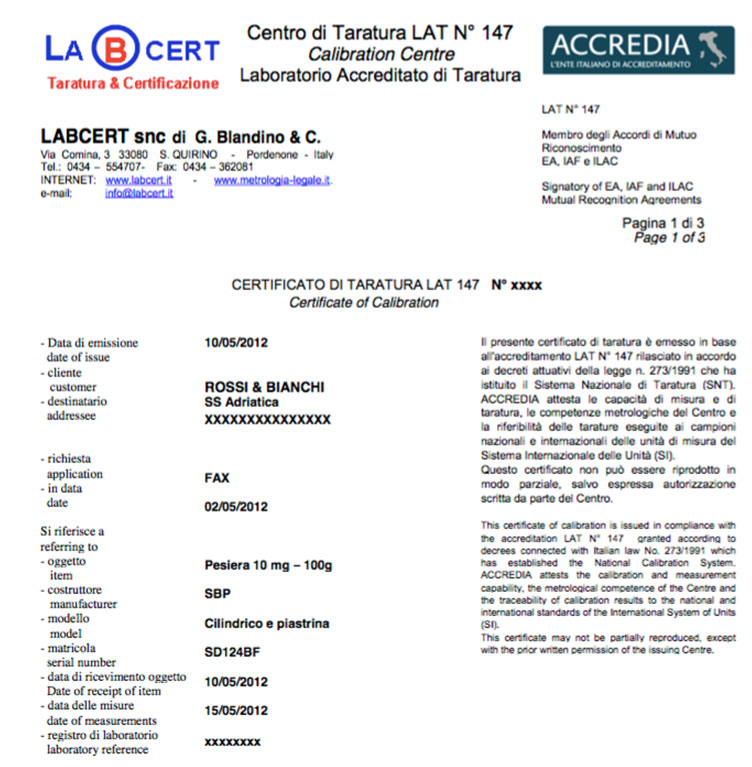
\includegraphics[width=0.5\linewidth]{fig/screenshot016}} \quad \subfloat{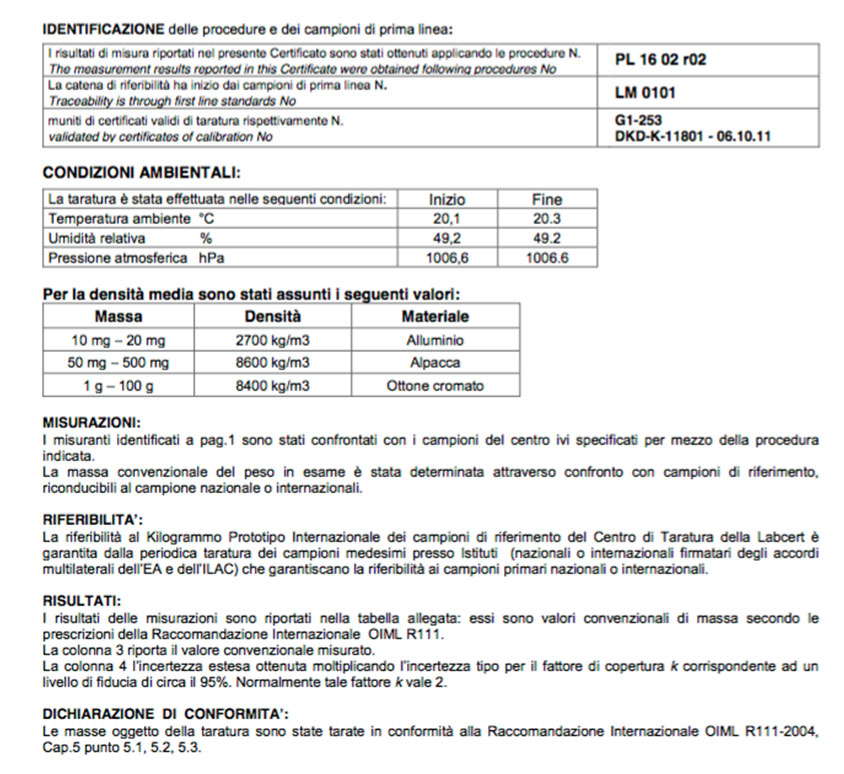
\includegraphics[width=0.5\linewidth]{fig/screenshot017}} \quad \subfloat{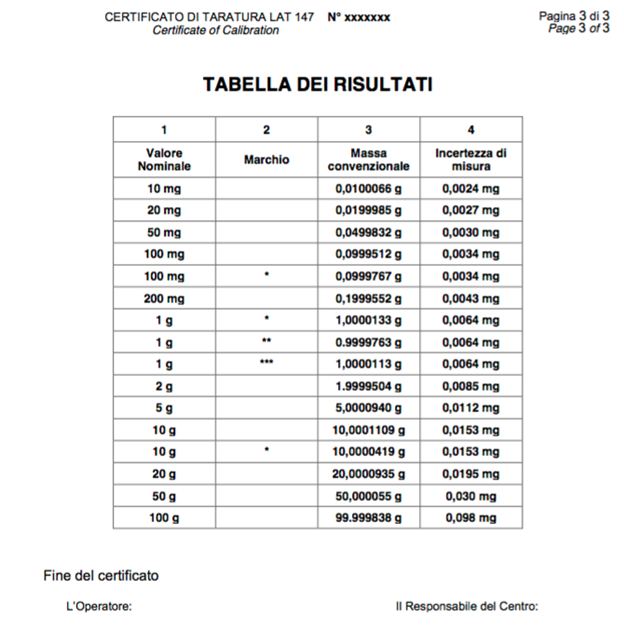
\includegraphics[width=0.5\linewidth]{fig/screenshot018}}
   	\end{figure}
   	
\newpage

{\LARGE \textbf{NOTE}}
	
	%DA DECOMMENTARE PER AVERE LA VERSIONE STAMPABILE A DUE PAGINE 	
	%	\newpage
	%		\null
	%		\vfill
	%\begin{tcolorbox}[height=4.5cm]
	%	This box has a height of 4.5cm.
	%\end{tcolorbox}
	%		

\end{document}